
\chapter{Shila - Introduction}
\label{chap:ShilaIntroduction}

This chapter introduces the reader with the central point of this thesis and the author's main contribution towards the establishment of a more secure internet architecture. A piece of software that allows the usage of MPTCP over SCION. The chapter includes a presentation of the software, an explanation of how users can use it and a rough outline of the functionality under the hood. A detailed discussion of the implementation and design decisions made follows in Chapter \ref{chap:ShilaImplementation}.   

\section{Introduction}
\label{sec:ShilaIntroduction}

Shila could very well be the name of the female lead role in a thrilling crime novel. However, in the context of this work Shila is the abbreviation of Shim Layer. It appropriately names the implementation which, by mediating between the two technologies, enables the use of MPTCP via SCION.

\subsection{Initial situation}
\label{subsec:ShilaInitialSituation}

To simplify the following descriptions, the starting point for the use of Shila is defined here. To use Shila, one needs at least two computers with MPTCP installed. In addition, the devices must be connected through the SCION network.\footnote{The usage of multiple instances of Shila on a single device is also possible. For illustrative purposes, however, this scenario is not discussed here.} Guidance to install MPTCP can be found here \cite{MPTCPWebMain}, the setup of SCION is described in detail on the official SCION webpage \cite{SCIONWebMain}.

Each computer is identified by a SCION address, not surprisingly referred as the SCON address of a host. TCP applications, or TCP endpoints, which are executed on a host are bound to a regular network interface. They are uniquely addressable through a IP address paired with a TCP port number, denoted as TCP address of an application. The individual parts of this tuple are called the IP address or the TCP port of an application. Furthermore, TCP endpoints can also be linked with addresses of the SCION namespace. The same principle applies here. Thus, an application may also be identified either by a full SCION address or just individual parts of it, e.g. just the SCION port.

\subsection{Usage}
\label{subsec:ShilaUsage}

In the following, we describe with a simple example case how a user can use Shila. An extensive description on how to use Shila with all its flags and settings is part of the code repository \cite{ShilaGithub}.

As an example, a setup with two endpoints is considered. Host 1 with SCION address 1-ff00:0:112,127.0.0.1 and Host 2 with SCION address 2-ff00:0:220,127.0.0.1, both part of the SCION network. The goal is to establish a connection between the client instance of an TCP application running on Host 1 and the respective server instance with TCP address 10.7.0.9:27041 running on Host 2. As an example TCP application, we consider iPerf3, the well-known measurement tool.

First, the so-called Routing-Information for the Shila instance running on Host 1 has to be prepared. It describes the mapping between TCP address of an application running on a certain host and this host's SCION address. The routing information is stored in a file is named \textit{routing.json} and is located in the Shila root directory. For the given example it contains only one entry:

\begin{minted}
{json}
[{ "key"  : { "ip" : "10.7.0.9", "port" : "27041" },
   "flow" : { "address"  : "2-ff00:0:220,127.0.0.1:27041" } }]
\end{minted}

In the second step, the Shila instance on both hosts can be started. If no arguments are specified the program starts with the default settings and loads the routing entries from the previously mentioned file:
\begin{minted}
{bash}
sudo ./shila
\end{minted}
The server instance of iPerf3 can be started on Host 2 once the shim layer is running. To be reachable the instance has to be started in the ingress network namespace of Shila:

\begin{minted}
{bash}
sudo ip netns exec shila-ingress iperf3 -s -p 27041
\end{minted}

As a final step the client part of iPerf3 is executed in Shilas egress network namespace on Host 1:

\begin{minted}
{bash}
sudo ip netns exec shila-egress iperf3 -c 10.7.0.9 -p 27041
\end{minted}

\newpage
We showcase the output of some of the involved entities. Figure \ref{fig:IntroductionOutputShilaOnHost1} displays the output generated by the Shila instance running on Host 1. The shim layer creates a default number of three paths through the SCION network used for the data exchange between the two iPerf3 instances. Figure \ref{fig:IntroductionOutputIperfOnHost1} shows the output generated by iPerf3 running on Host 1. Figure \ref{fig:IntroductionDataDistributionAmongPaths} visualizes the distribution of the data exchange among the three different flows generated from a packet capturing.

\begin{figure}
	\begin{center}
		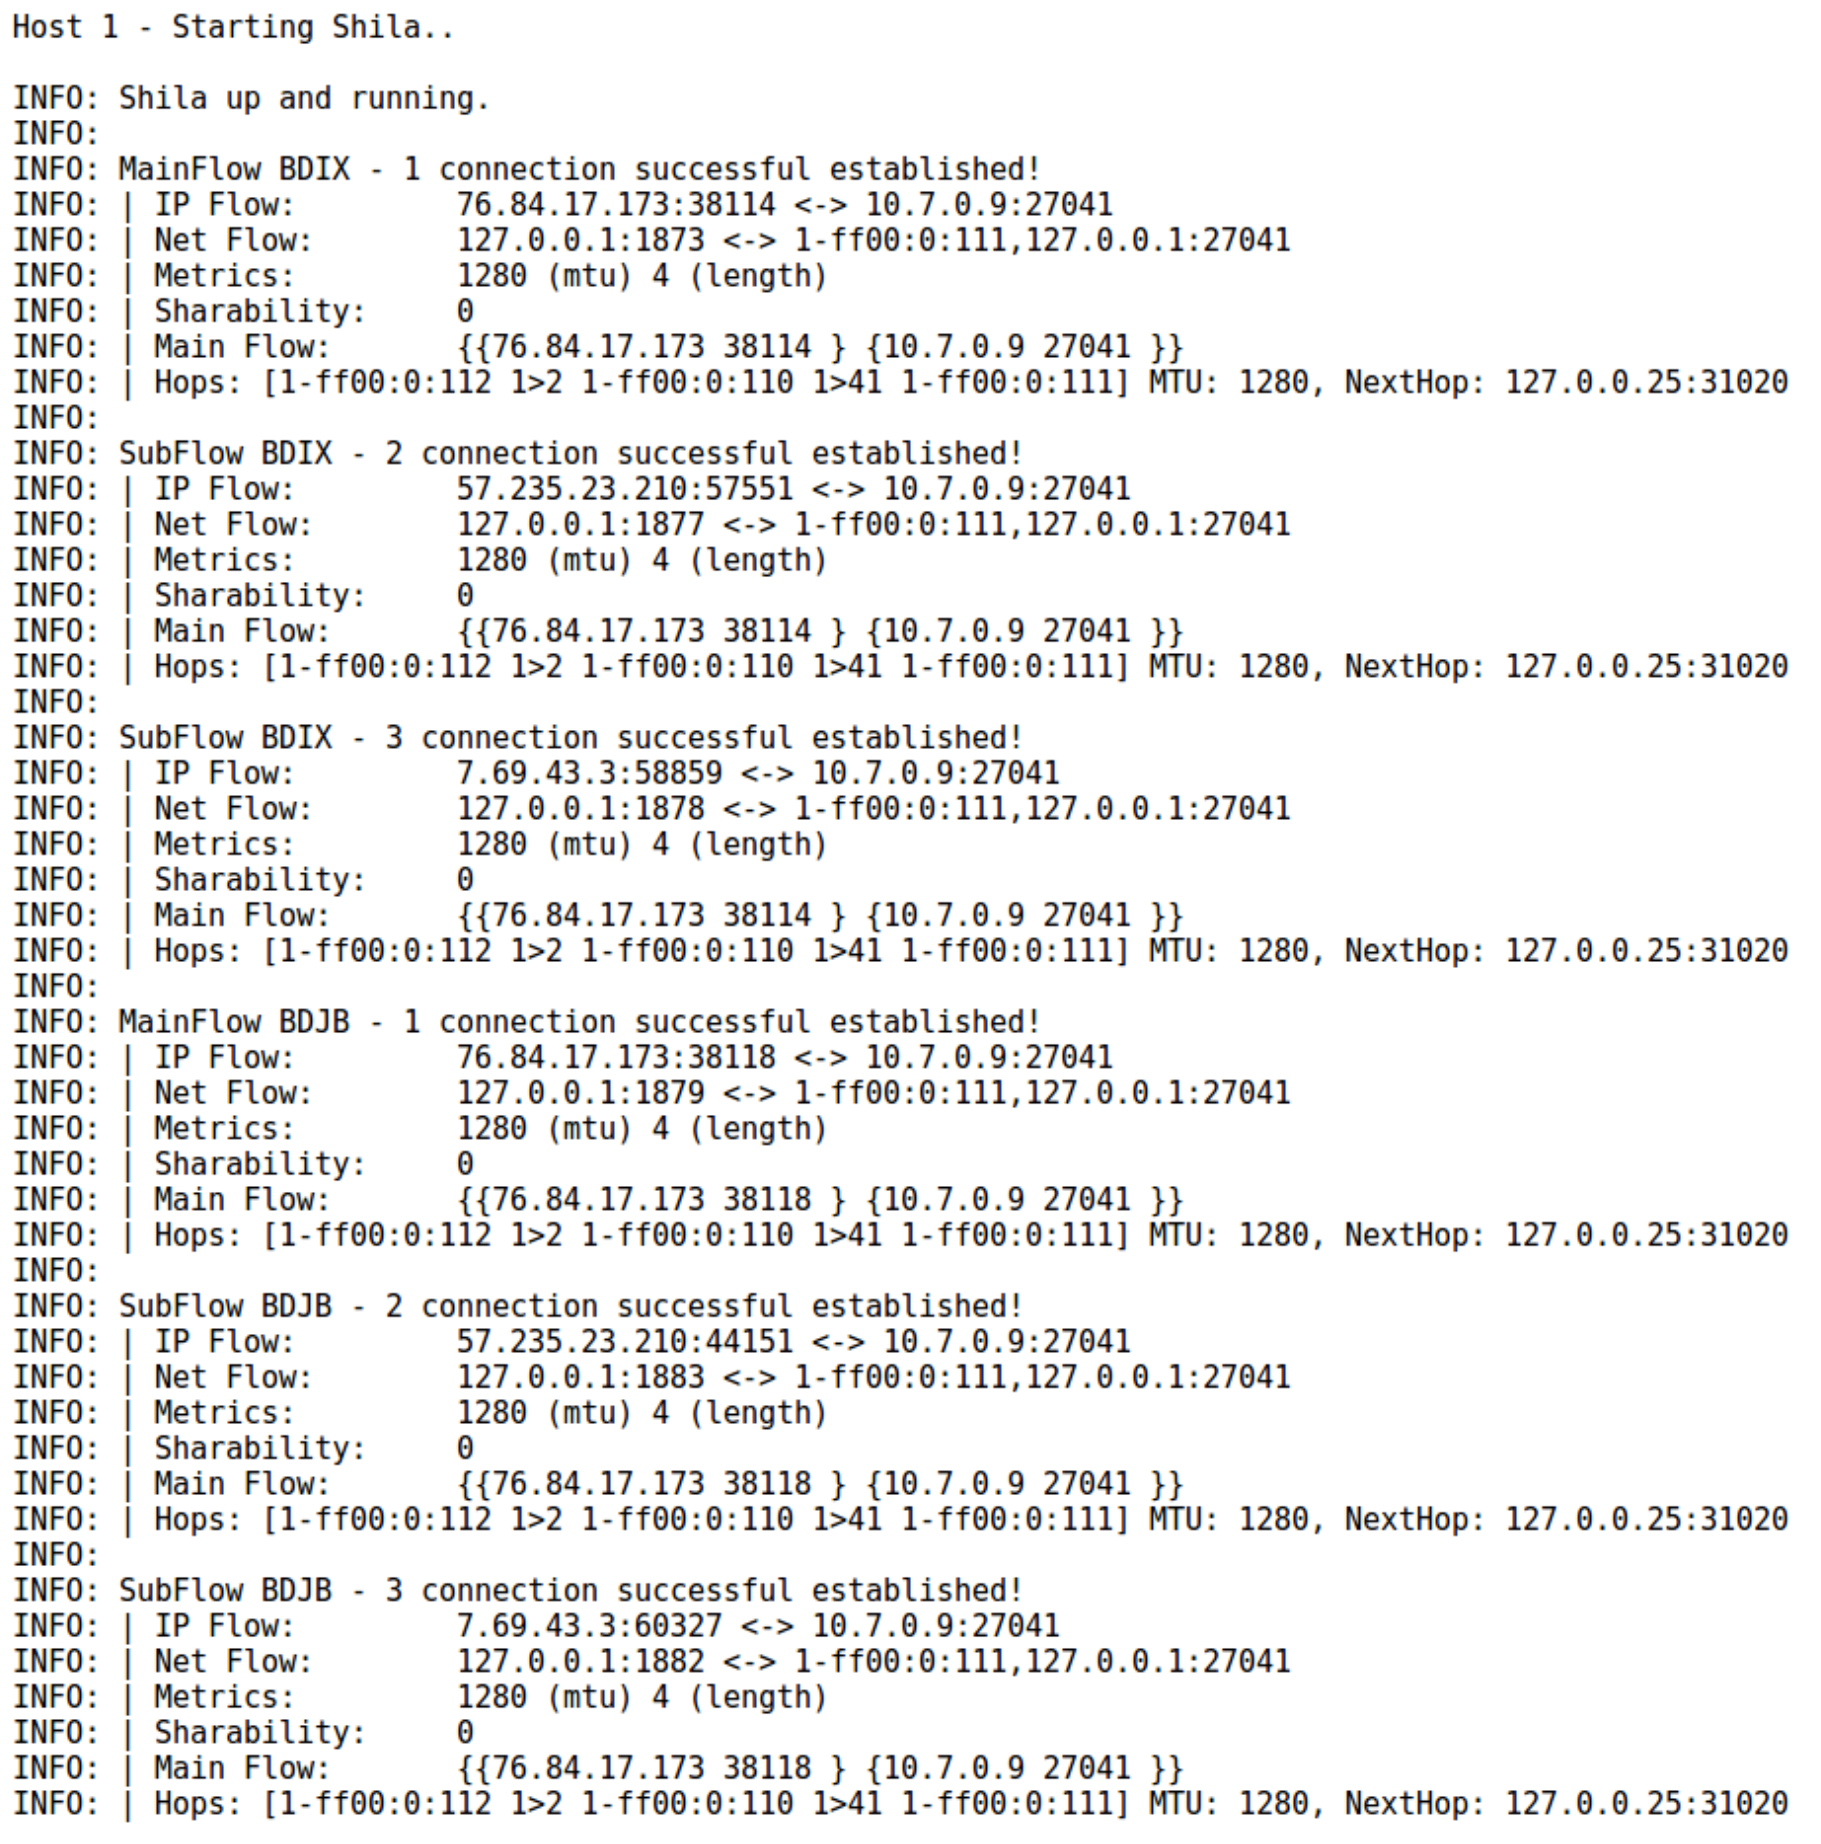
\includegraphics[scale=0.27]{../illustrations/shilaIntroduction/OutputShilaHost1.pdf}  
		\caption[Caption for the list of figures.]{Output generated by the Shila instance running on Host 1. Note that iPerf3 creates two TCP connections, one to send the control signals and one for the actual data exchange.}
		\label{fig:IntroductionOutputShilaOnHost1}
	\end{center}
\end{figure}

\begin{figure}
	\begin{center}
		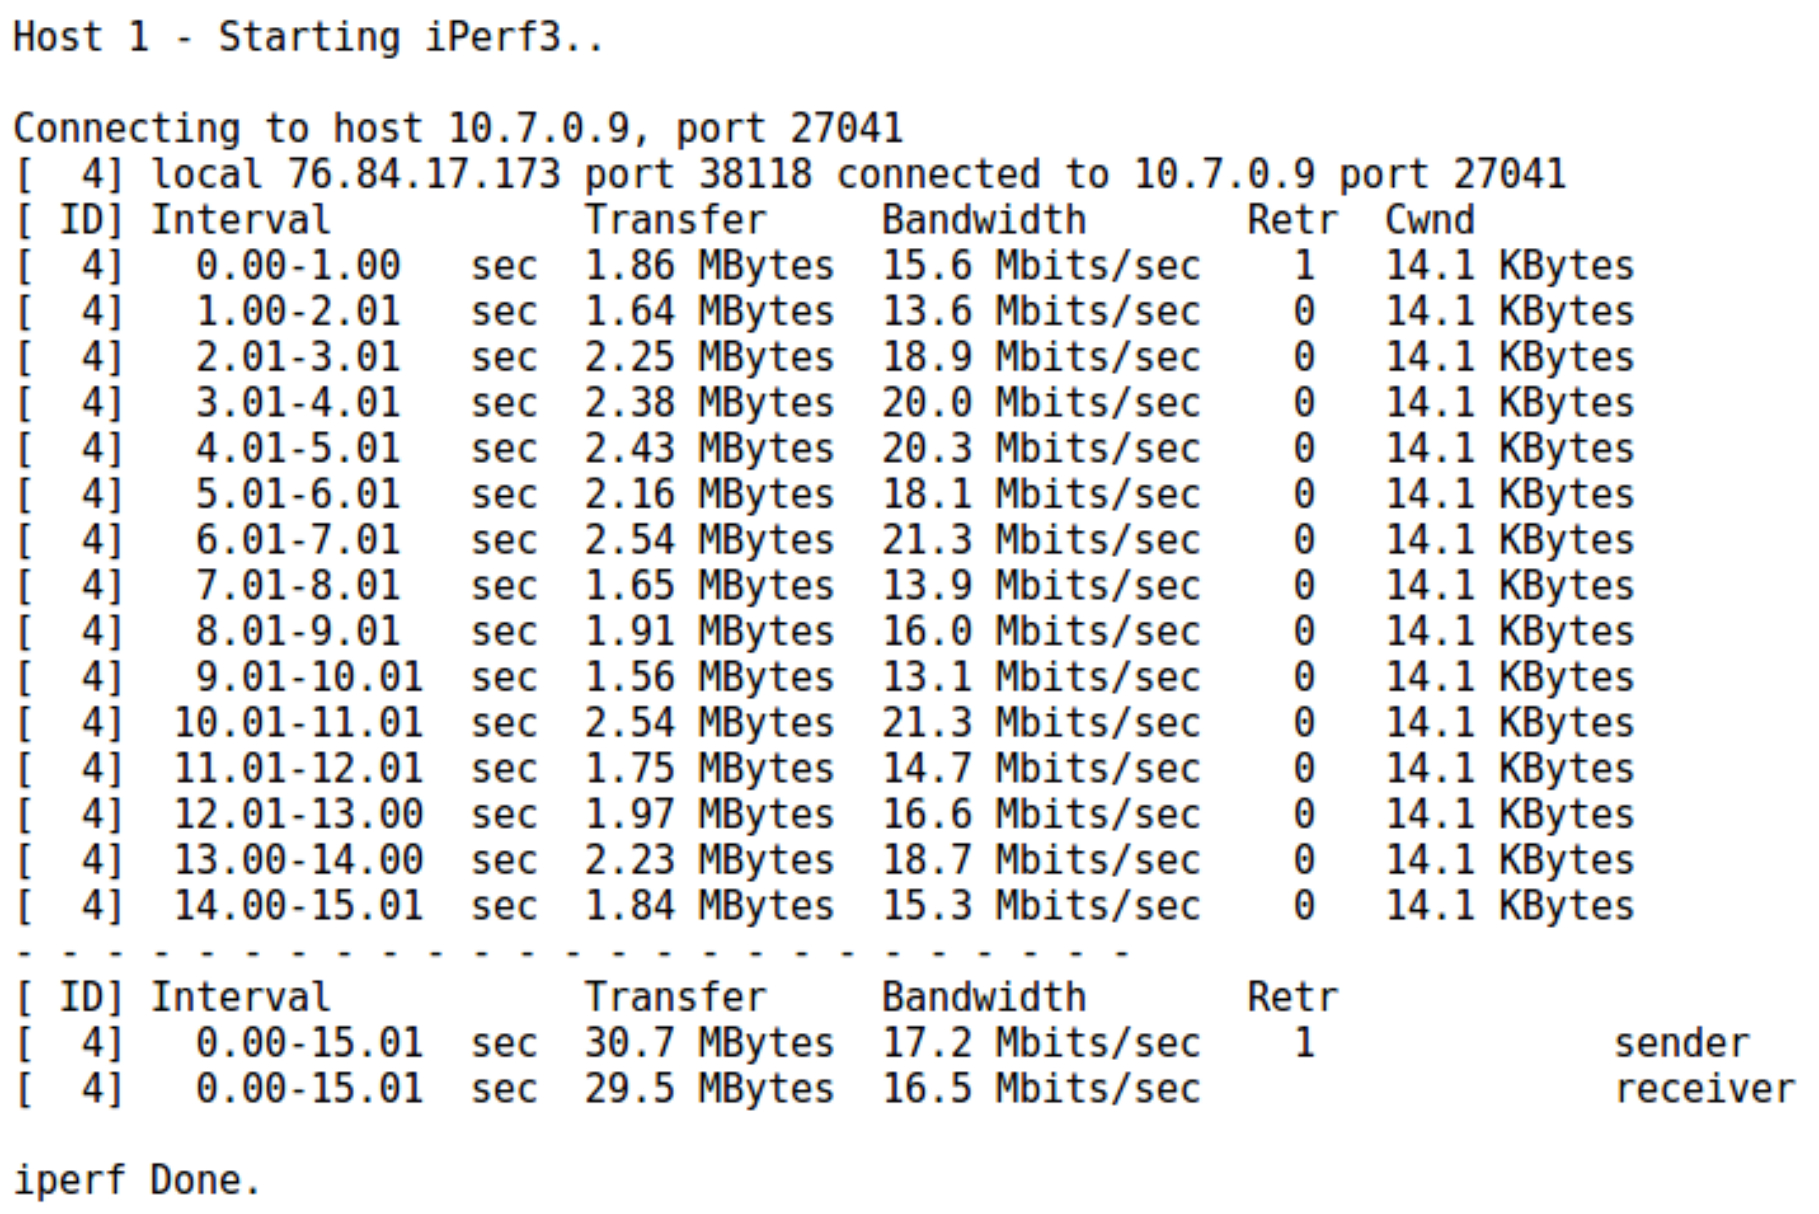
\includegraphics[scale=0.27]{../illustrations/shilaIntroduction/OutputiPerf3Host1.pdf}  
		\caption[Caption for the list of figures.]{Output generated by the iPerf3 client instance on Host 1. Note that the measured metrics are not representative since the test run was done on a local setup of SCION.}
		\label{fig:IntroductionOutputIperfOnHost1}
	\end{center}
\end{figure}

\begin{figure}
	\begin{center}
		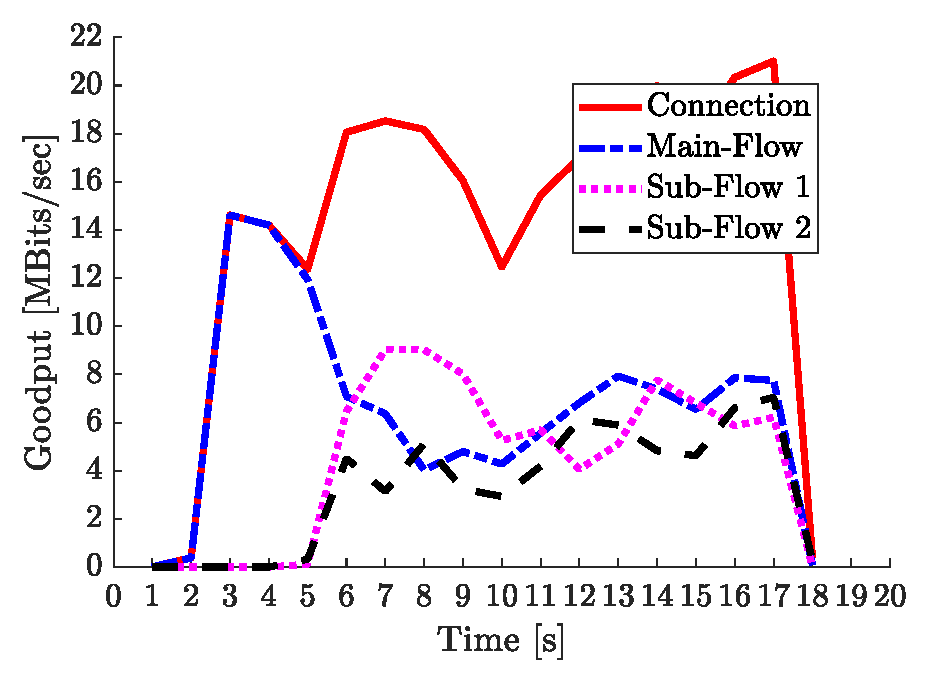
\includegraphics[scale=0.65]{../illustrations/shilaIntroduction/DistributionOfFlows.eps}  
		\caption[Caption for the list of figures.]{Plot showing how the achieved goodput for the connection between Host 1 and Host 2 is under hood distributed to the three flows created by Shila.}
		\label{fig:IntroductionDataDistributionAmongPaths}
	\end{center}
\end{figure}


\newpage
\section{Functionality}
\label{sec:ShilaFunctionality}

The functionality of Shila can be divided into three parts. The first part considers the setup of Shila in general, i.e. everything necessary to get a running instance of Shila. The latter two parts specifically consider the data exchange between two TCP endpoints. The second part discusses what is necessary to establish such a connection and the third part covers the operating state but also the cleaning up once a connection is no longer needed. 

In the following, we will treat these three parts for the first time, so that the reader gets a good basic understanding of the mechanics of Shila. In chapter \ref{chap:ShilaImplementation} everything mentioned is explained again in more detail.

\subsection{Setup}
\label{subsec:ShilaSetup}

Launching and setting up Shila includes the following steps.

\paragraph{Loading of the Routing-Information} Shila reads the Routing-Information presented in the respective file. It contains the mapping from TCP addresses of applications to SCION addresses of hosts running these apps. 

\paragraph{Setup of Namespaces} Shila sets up two different network namespaces. The ingress namespace holds the network interface used to accept incoming connections. The egress namespace accommodates the network interfaces which are used for connections initiated by the respective host.

\paragraph{Creation of virtual Interfaces} A virtual network interface is a network device that is supported entirely in software, i.e. there is no real hardware network adapter. It allows applications to take over the role of the wire. For a real network interface, the IP datagrams of connected applications are sent directly to the cable. Virtual interfaces make these data available to applications in userspace.

The shim layer instantiates a single virtual network interface in the ingress namespace. This interface is per default bound to the IP address 10.7.0.9 and is used by all listening TCP applications to bind their sockets. In the egress namespace one to eight\footnote{The current implementation of MPTCP uses a maximum of eight different interfaces for a single MPTCP connection.} virtual interfaces can be instantiated, where each is assigned a random IP address. Each of these virtual network interfaces later corresponds to a single path of an MPTCP connection.

\paragraph{Running the Contact-Server-Endpoint} To be receptive to incoming connections Shila starts a so-called Contact-Server-Endpoint. It binds per default to the SCION port 7654 and serves as an initial point of contact. Shila instances running on different hosts initiate possible data exchange through this contact point.

\begin{figure}
	\begin{center}
		\def\svgwidth{1\textwidth}
		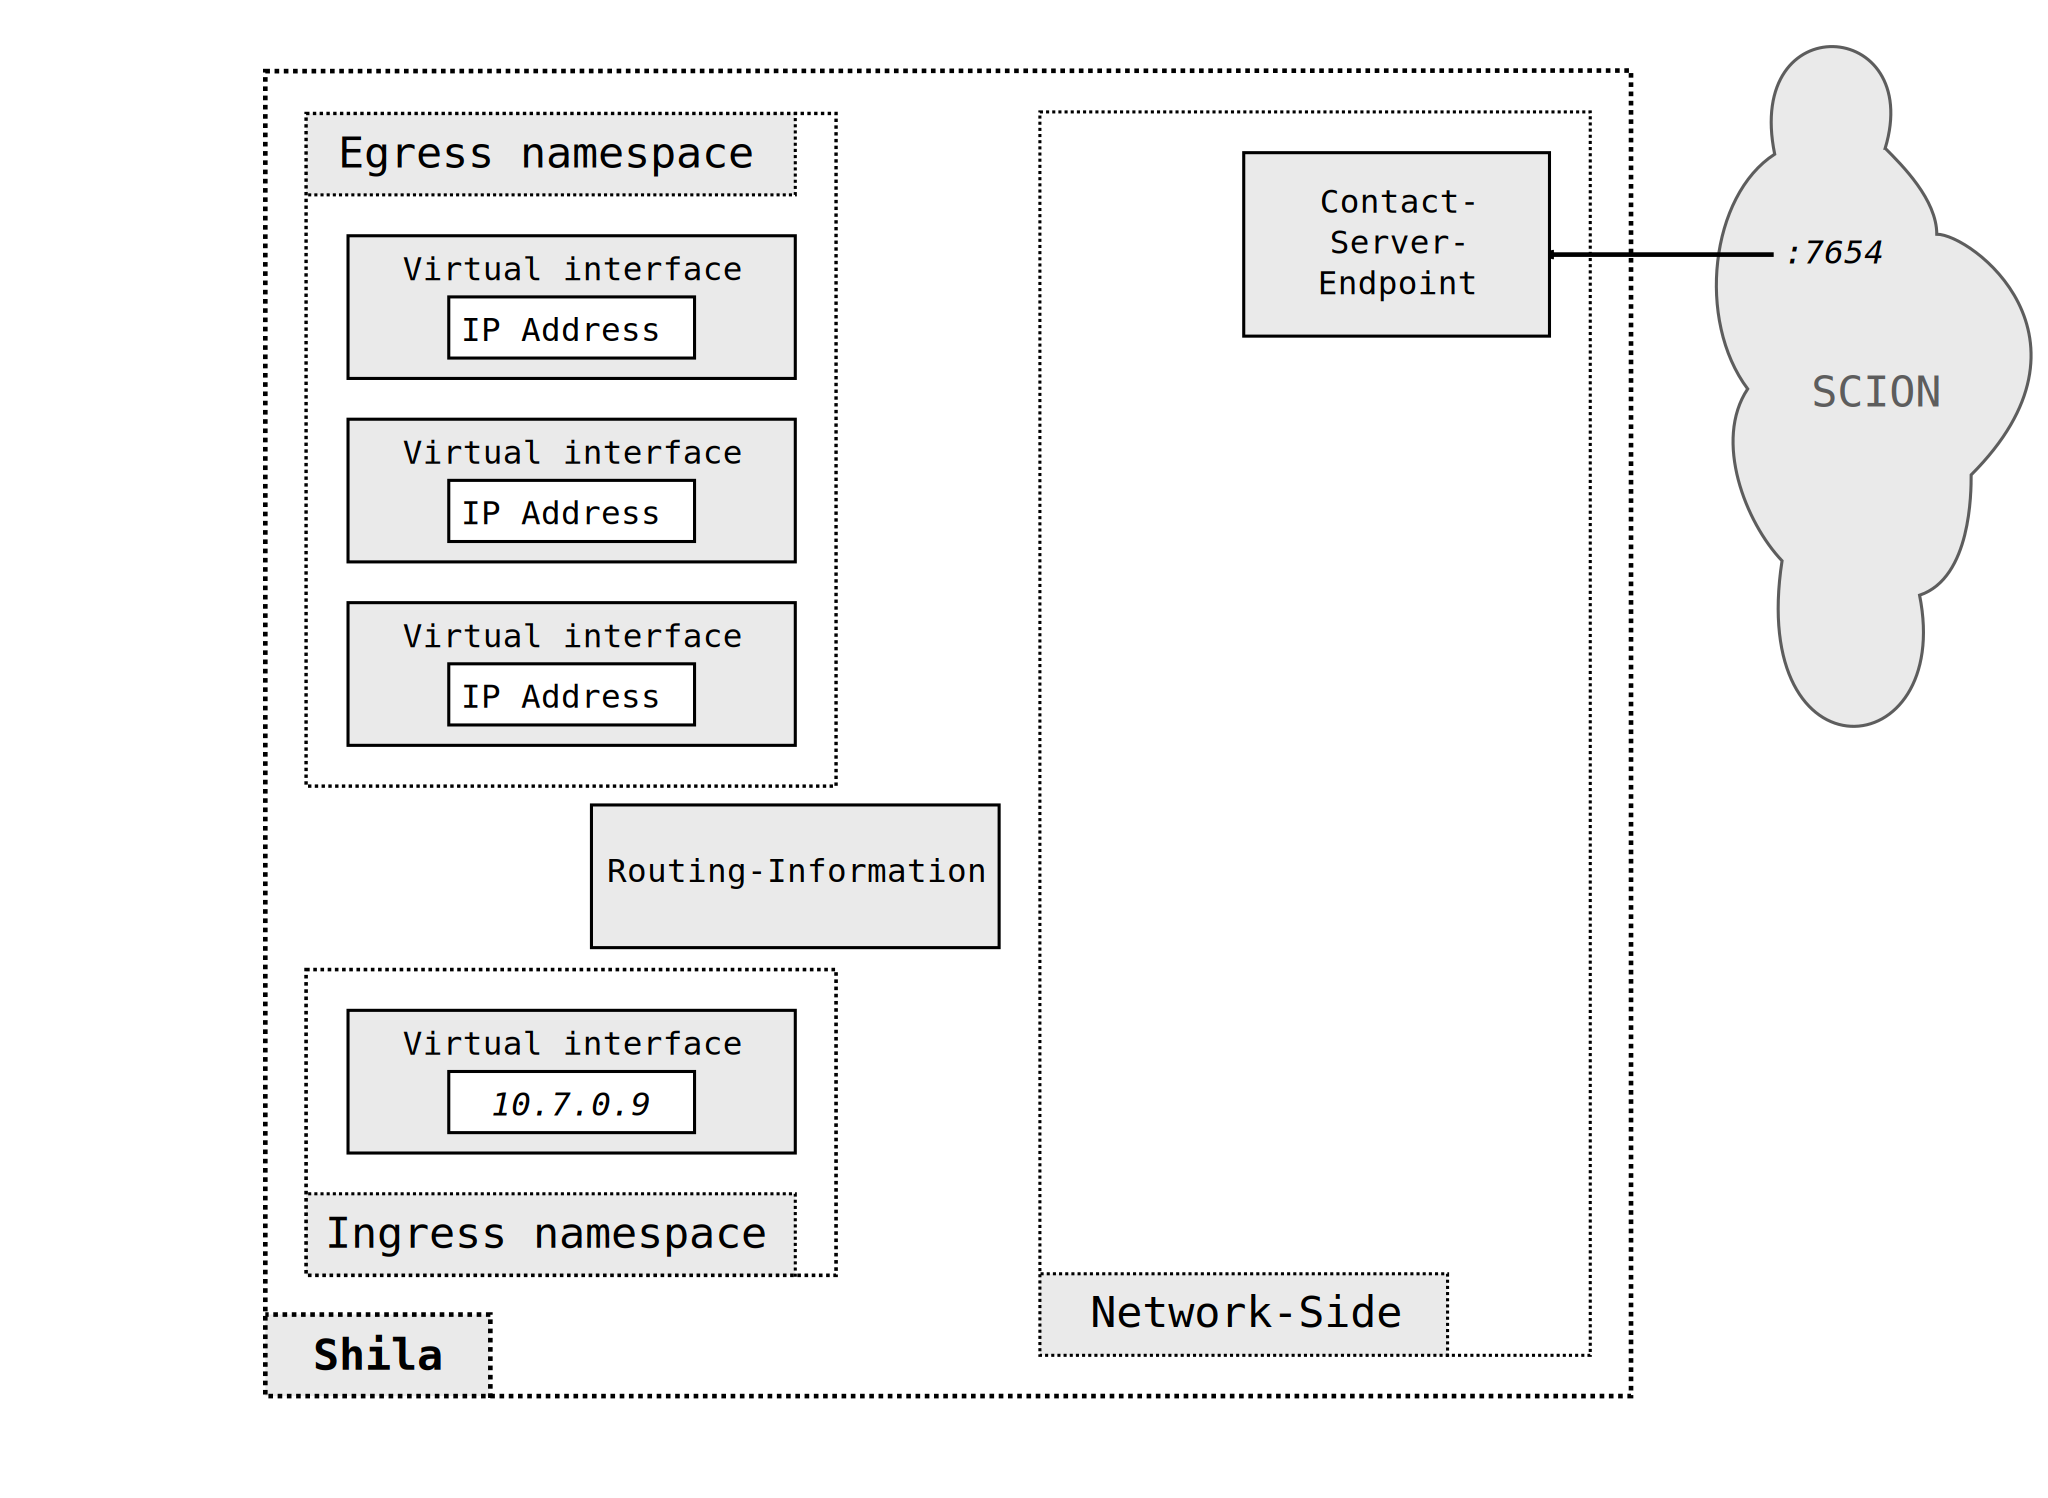
\includegraphics[scale=0.2]{../illustrations/shilaIntroduction/StateAfterSetup.pdf}   
		\caption[Caption for the list of figures.]{Illustration of the state of Shila once setup is complete.}
		\label{fig:ShilaIllustrationStateAfterSetup}
	\end{center}
\end{figure}

Figure \ref{fig:ShilaIllustrationStateAfterSetup} illustrates the state of Shila once the setup has completed. The implementation is now ready to establish connections and provide data exchange between client and server instance of TCP applications running on, possibly different, SCION hosts. 

\subsection{Connection Establishment}
\label{subsec:ShilaConnectionEstablishment}

This Subsection presents the individual steps of a connection establishment between a client instance of an application and its server counterpart over MPTCP on top of SCION. The discussion is based on the example of Subsection \ref{subsec:ShilaUsage} and it assumes that a successfully initialized instance of Shila is running on Host 1 and Host 2. All the presented steps are illustrated in Figure \ref{fig:ShilaIllustrationConnectionEstablishment}. 

\begin{figure}
	\begin{center}
		\def\svgwidth{1\textwidth}
		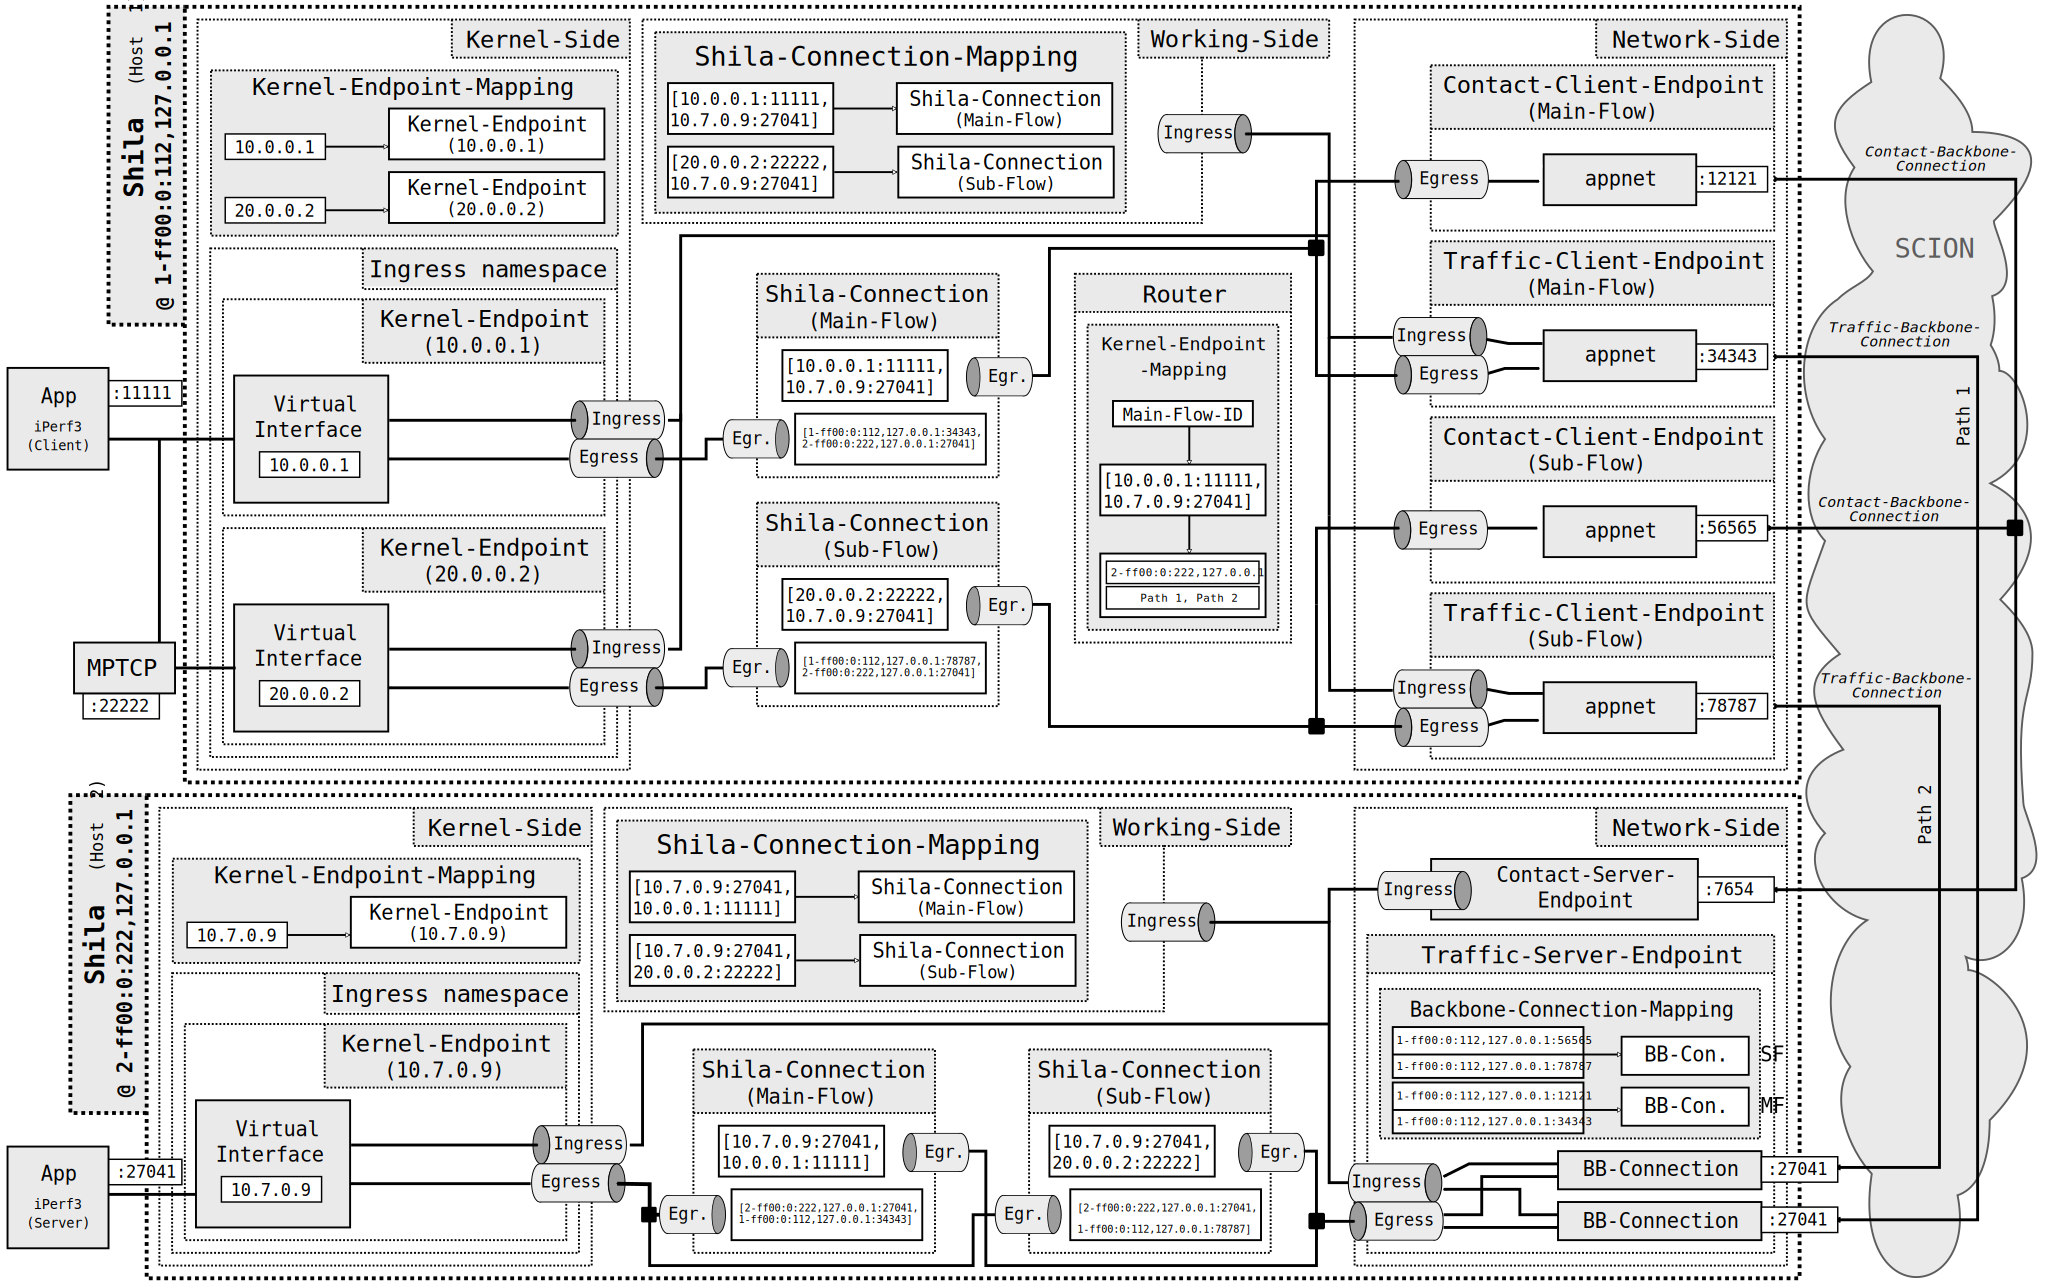
\includegraphics[scale=0.2]{../illustrations/shilaIntroduction/ConnectionEstablishment.pdf}   
		\caption[Caption for the list of figures.]{Illustration of the steps involved in the connection establishment of a Main-Flow (\textbf{M-1} to \textbf{M-10}) and a Sub-Flow (\textbf{S-1} to \textbf{S-10}).}
		\label{fig:ShilaIllustrationConnectionEstablishment}
	\end{center}
\end{figure}

The creation of a connection itself can be divided into two parts. The establishment of the initial TCP connection, also called Main-Flow, and the establishment of further TCP connections, the so-called Sub-Flows. In the rest of this work, a connection always means the totality of all flows, i.e. the Main-Flow and all possible Sub-Flows. Let us start with a walk-through through the sequence of steps of a Main-Flow establishment.

\textbf{Main-Flow Establishment}

\begin{description}
	\item[M-1] On Host 2, the server instance of iPerf3 starts listening for incoming TCP connections. It therefore binds to the virtual interface in the Shila ingress namespace on the TCP address 10.7.0.9:27041. This step is not recognized by Shila.
	\item[M-2] On Host 1, the client instance of iPerf3 tries to connect to its server counterpart on TCP address 10.7.0.9:27041. For the connection establishment an IP datagram, containing the TCP-SYN, is sent via one of the virtual interfaces in the egress namespace where it is intercepted by Shila.
	\item[M-3] Shila extracts the destination TCP address from this datagram and looks up the corresponding SCION address in the Routing-Information. For the example, this is 2-ff00:0:220,127.0.0.1, the SCION address of Host 2. 
	\item[M-4] A Contact-Client-Endpoint is created. It establishes a backbone connection, called Contact-Backbone-Connection, over SCION to the Contact-Server-Endpoint listening on Host 2, SCION port 7654.
	\item[M-5] The TCP-SYN is forwarded to the server along the Contact-Backbone-Connection.
	\item[M-6] The Shila instance on the server-side hands over the received IP datagram, holding the TCP-SYN, to the virtual network interface in the ingress namespace. From there the datagram finds its destination, the iPerf3 server instance.
	\item[M-7] On Host 2, a Traffic-Server-Endpoint, listening on SCION port 27041, is created, ready to receive backbone connections.
	\item[M-8] On Host 1, a Traffic-Client-Endpoint is created. It establishes a so-called Traffic-Backbone-Connection to its counterpart on the server-side.
	\item[M-9] The IP datagram containing the answer from the iPerf3 server instance, a TCP-SYN+ACK, arrives at the Shila instance on Host 2. It is forwarded to the corresponding Traffic-Server-Endpoint. From there it is sent over the Traffic-Backbone-Connection to Host 1.
	\item[M-10] The reception of the first data received from the Traffic-Client-Endpoint on Host 1 concludes the establishment of the Main-Flow. Shila extracts its identifier, denoted as Main-Flow-Identifier, and links it to the corresponding routing information. This mapping is important for the following creation of Sub-Flows. The IP datagram, holding the TCP-SYN+ACK, is finally handed to the virtual interface from where the initial TCP-SYN came from. From there it finds its way to the client instance of iPerf3.
\end{description}

As soon as the Main-Flow of a connection is established, MPTCP starts to build Sub-Flow. The procedure differs only in some points from the procedure for establishing a Main-Flow. These points are mentioned below. For illustration purposes, an established Sub-Flow is indicated in Figure \ref{fig:ShilaIllustrationConnectionEstablishment}.

\textbf{Sub-Flow Establishment}

\begin{description}
	\item[(S-1)] This step is not necessary, the server-side of the app is still listening.
	\item[S-2] The initial connection request for a Sub-Flow is not made by the client instance of the application but by MPTCP itself.
	\item[S-3] For a Sub-Flow, Shila extracts the identifier for the corresponding Main-Flow, i.e. the Main-Flow-Identifier, which is carried in the  TCP-SYN datagram. It uses this identifier to get all the necessary information about the connection, e.g. the SCION destination address, from the Routing-Information.
	\item[S-7] For a Sub-Flow it is not necessary to create a new Traffic-Server-Endpoint which listens on SCION port 27041. Such an instance was already created during the establishment of the corresponding Main-Flow.
\end{description} 

Once established, a flow is immediately used for the data exchange of the application. If at one point the connection is no longer needed, it is removed again, as mentioned in the following subsection \ref{subsec:ShilaCleanUp}.

\subsection{Normal Operation and Clean-Up}
\label{subsec:ShilaCleanUp}

As soon as the Main-Flow or a Sub-Flow is established, its Contact-Backbone-Connection is no longer needed and is terminated. For data exchange between the TCP endpoints, data can be forwarded through all established flows. The decision along which flow the data is sent is made by MPTCP and cannot be influenced by Shila. Data forwarded along a certain flow travels via the respective endpoints along the Traffic-Backbone-Connection through the SCION network.  If a connection is no longer needed, i.e. no more data is flowing through its flows, then the respective Traffic-Backbone-Connections are removed together with its endpoints.
